
\documentclass[twocolumn]{article}

\usepackage{amsmath}
\usepackage{graphicx}
\usepackage{times}

\title{Exploration of the Parameter Space for an Inclined-Plane Problem}

\begin{document}

\maketitle

\begin{abstract}
   A moderately complex problem involving a block sliding on an inclined plane,
   a pulley with rotational inertia, and a second block serving as a
   counterweight is solved. We present the proper approach, in which no
   numerical value for any parameter is assumed in the solution. Then the
   limiting cases are explored. Finally, a summary of the parameter space is
   presented in a collection of graphs.
\end{abstract}

\section{Problem}

\begin{figure*}
   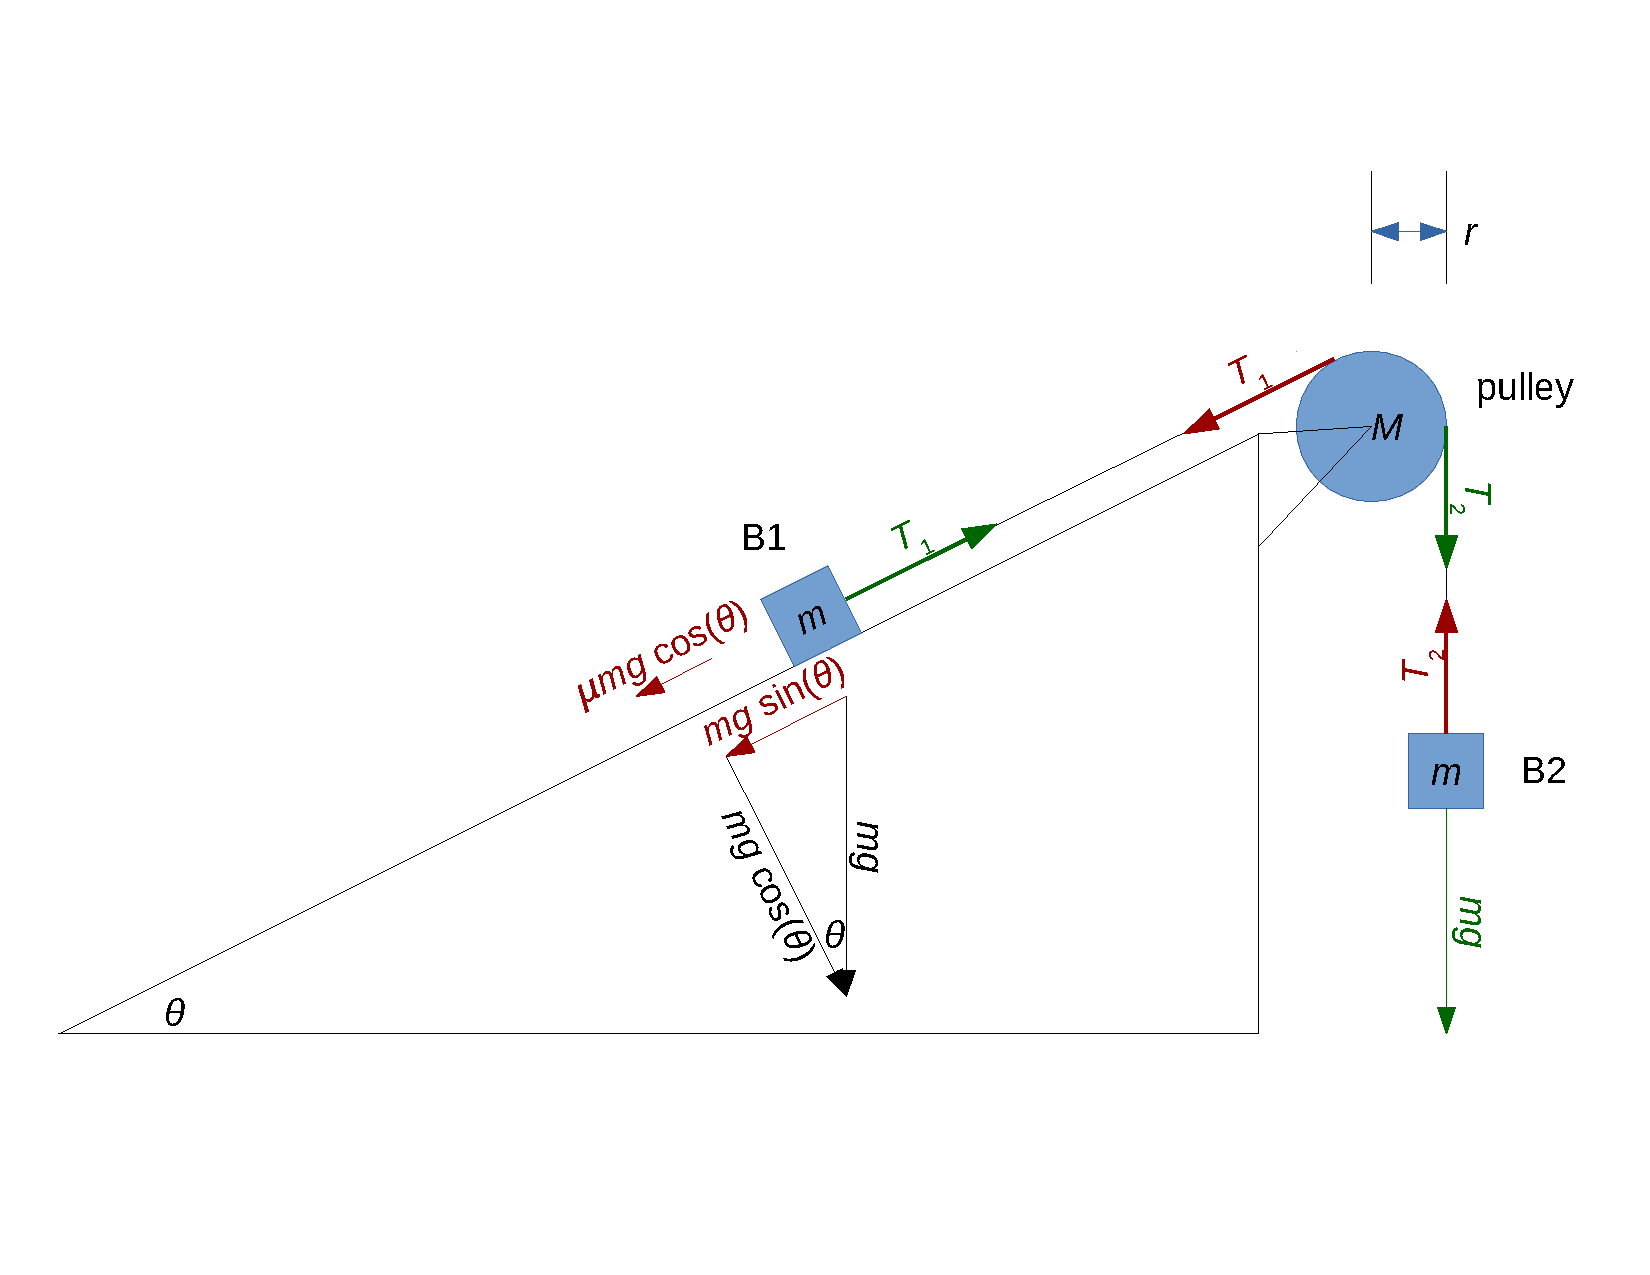
\includegraphics[width=\textwidth]{diagram}
   \caption{Diagram of problem.}
   \label{fig:diagram}
\end{figure*}

The flat bottom of a block B1 of mass~$m$ lies on a plane inclined at an
angle~$\theta$ to the horizontal. See Figure~\ref{fig:diagram}. The coefficient
of kinetic friction between the plane and the block is $\mu$.  A massless,
taut, inelastic cable runs from B1 toward the top of the plane, around a
pulley, and straight down to another block B2, which also has mass~$m$.  The
pulley's disc has infinite static friction against the cable but requires no
energy to separate from the cable as it moves. The pulley's bearing is
frictionless. The disc of the pulley has uniform density, total mass $M$, and
radius $r$. Find the acceleration $a$ of the blocks; express $a$ in terms of
$\mu$, $m$, $M$, $\theta$, and the acceleration $g$ of gravity.

\section{Solution}

Each of B1, the pulley, and B2 must undergo the same acceleration because they
move as a rigid system: B1 and B2 maintain a constant distance of separation
along the length of the cable, and the cable does not slip along the surface of
the pulley.  The net force on each of B1, the pulley, and B2, when divided by
the relevant mass, must yield the same acceleration.

\subsection{Forces at B1}

Suppose that the tension in the cable attached to B1 is $T_1$. There are three
forces, parallel to the plane, acting on B1:
\begin{enumerate}
      \item a force of magnitude $T_1$ toward the pulley,
      \item the frictional force $\mu m g \cos(\theta)$ away from the pulley,
         and
      \item the plane-parallel component $m g \sin(\theta)$ of B1's weight.
\end{enumerate}
The acceleration, as derived from forces acting on B1, is
\begin{eqnarray}
   \nonumber
   a &=& \frac{T_1 - \mu m g \cos(\theta) - m g \sin(\theta)}{m}\\
   a &=& \frac{T_1}{m} - [\mu \cos(\theta) + \sin(\theta)] g.
   \label{eq:B1}
\end{eqnarray}

\subsection{Forces at the Pulley}

Suppose that the tension in the cable attached to B2 is $T_2$. There are two
forces, along the direction of the cable, acting on the pulley:
\begin{enumerate}
   \item a force of magnitude $T_1$ toward B1 and
   \item a force of magnitude $T_2$ toward B2.
\end{enumerate}
There are two corresponding torques:
\begin{enumerate}
   \item a torque $r T_1$ tending to spin the pulley so that B1 accelerates
      down the plane and
   \item a torque $r T_2$ tending to spin the pulley so that B1 accelerates up
      the plane.
\end{enumerate}
The angular acceleration, derived from torques acting on the pulley, is
\begin{eqnarray}
   \nonumber
   \alpha &=& \frac{r T_2 - r T_2}{\tfrac{1}{2} M r^2}\\
   \alpha &=& \frac{2 \: [T_2 - T_1]}{M r}.
\end{eqnarray}
The acceleration, as derived from forces acting on the pulley, is
\begin{eqnarray}
   \nonumber
   a &=& r \alpha\\
   a &=& \frac{2 \: [T_2 - T_1]}{M}.
   \label{eq:pulley}
\end{eqnarray}

\subsection{Forces at B2}

There are two forces acting on B2:
\begin{enumerate}
   \item a force of magnitude $T_2$ toward the pulley and
   \item B2's weight $mg$ away from the pulley.
\end{enumerate}
The acceleration, as derived from forces acting on B2, is
\begin{eqnarray}
   \nonumber
   a &=& \frac{mg - T_2}{m}\\
   a &=& g - \frac{T_2}{m}.
   \label{eq:B2}
\end{eqnarray}

\subsection{Tension Acting on B2}

We can, by combining Equation~\ref{eq:pulley} and Equation~\ref{eq:B2}, solve
for the tension $T_2$ acting on B2.
\begin{eqnarray}
   \nonumber
   \frac{2 \: [T_2 - T_1]}{M} &=& g - \frac{T_2}{m}\\
   \nonumber
   \frac{2 \: T_2}{M} + \frac{T_2}{m} &=& g + \frac{2 \: T_1}{M}\\
   \nonumber
   \left[ \frac{2}{M} + \frac{1}{m} \right] T_2 &=& g + \frac{2 \: T_1}{M}\\
   \nonumber
   \left[ 2 + \frac{M}{m} \right] T_2 &=& M g + 2 \: T_1\\
   T_2 &=& \frac{M g + 2 \: T_1}{2 + \tfrac{M}{m}}
   \label{eq:T2}
\end{eqnarray}
Here we have expressed the result in terms of the ratio $\tfrac{M}{m}$, which,
along with $\mu$ and $\theta$, is one of the three fundamental parameters that
determine the solution.

\subsection{Tension Acting on B1}

Now, combining Equation~\ref{eq:B1}, Equation~\ref{eq:B2}, and
Equation~\ref{eq:T2}, we can solve for the tension $T_1$ acting on B1.
\begin{eqnarray}
   \nonumber
   g - \frac{T_2}{m} &=& \frac{T_1}{m} - [\mu \cos(\theta) + \sin(\theta)] g\\
   \nonumber
   \frac{T_1 + T_2}{mg} &=& 1 + \mu \cos(\theta) + \sin(\theta)\\
   \nonumber
   \frac{T_1}{mg} \left[ \frac{4 + \tfrac{M}{m}}{2 + \tfrac{M}{m}} \right] &=&
   \frac{2}{2 + \tfrac{M}{m}} + \mu \cos(\theta) + \sin(\theta)
\end{eqnarray}
\begin{equation}
   T_1 = \left[ \frac{2 + [\mu \cos(\theta) + \sin(\theta)][2 +
   \tfrac{M}{m}]}{4 + \tfrac{M}{m}} \right] mg
   \label{eq:T1}
\end{equation}

\subsection{Acceleration of Blocks}

Finally, combining Equation~\ref{eq:T1} and Equation~\ref{eq:B1}, we can solve
for the acceleration.
\begin{small}
\begin{equation*}
   \frac{a}{g} = \frac{2 + [\mu \cos(\theta) + \sin(\theta)][2 +
   \tfrac{M}{m}]}{4 + \tfrac{M}{m}} - [\mu \cos(\theta) + \sin(\theta)]
\end{equation*}
\end{small}
\begin{equation}
   \frac{a}{g} = \left[ \frac{2}{4 + \tfrac{M}{m}} \right] [1 - \mu
   \cos(\theta) - \sin(\theta)]
\end{equation}
Again, we see that the acceleration depends on three parameters:
$\tfrac{M}{m}$, $\mu$, and $\theta$. The form of the solution shows that the
acceleration can range from a minimum of zero to a maximum of $\tfrac{g}{2}$.

\subsubsection{Minimum Acceleration}

The minimum ($a = 0$) obtains when either of the following is true:
\begin{itemize}
   \item $\tfrac{M}{m}$ approaches infinity, or
   \item $\mu \cos(\theta) + \sin(\theta) \geq 1$.
\end{itemize}
Considering the second case, we see that, for a given $\theta$, when $\mu$ is
larger than $\mu_\text{max} = \sec(\theta) - \tan(\theta)$, the kinetic
friction is large enough to decelerate the system and halt motion.
\begin{figure}
   \includegraphics[width=\columnwidth]{max-mu.png}
   \caption{Plotted against the angle of inclination of the plane, the limiting
   value $\mu_\text{max}$ of the coefficient of kinetic friction. For any
   coefficient above this limit, the system decelerates.}
   \label{fig:mu-max}
\end{figure}
Figure~\ref{fig:mu-max} shows the how $\mu_\text{max}$ varies with $\theta$.
For small $\theta$, $\mu$ can approach unity, and the system will still
accelerate. For values of $\theta$ approaching 90~degrees, however, only a
small $\mu$ allows the system to accelerate.

\subsubsection{Maximum Acceleration}

The maximum ($a = \tfrac{g}{2}$) obtains when all of the following are true at
the same time:
\begin{itemize}
   \item $\tfrac{M}{m}$ approaches zero;
   \item $\mu = 0$; and
   \item $\theta = 0$.
\end{itemize}

\subsubsection{Summary}

\begin{figure*}
   \includegraphics[width=\textwidth]{accel-001.png}
   \caption{Contour map showing lines of constant acceleration across the space
   of inclination angle and coefficient of kinetic friction for $\tfrac{M}{m} =
   0.1$. The value of each contour is labeled as a fraction of $g$.}
   \label{fig:accel-001}
\end{figure*}

\begin{figure*}
   \includegraphics[width=\textwidth]{accel-010.png}
   \caption{Contour map showing lines of constant acceleration across the space
   of inclination angle and coefficient of kinetic friction for $\tfrac{M}{m} =
   1.0$. The value of each contour is labeled as a fraction of $g$.}
   \label{fig:accel-010}
\end{figure*}

\begin{figure*}
   \includegraphics[width=\textwidth]{accel-100.png}
   \caption{Contour map showing lines of constant acceleration across the space
   of inclination angle and coefficient of kinetic friction for $\tfrac{M}{m} =
   10.0$. The value of each contour is labeled as a fraction of $g$.}
   \label{fig:accel-100}
\end{figure*}

Figure~\ref{fig:accel-001},~\ref{fig:accel-010}, and~\ref{fig:accel-100}
summarize the result.

\end{document}

